\chapter{Results}

Performing optimal control of quantum many-body systems is typically extremely resource demanding \cite{Mennemann2015}. Hence, previous studies of optimization of Bose-Hubbard dynamics have abstained from using gradient-based techniques and instead opted for the gradient-free Nelder-Mead method combined with control parameterizations \cite{Doria2011,FrankBloch}. The framework presented in this thesis combines tensor description of lattice systems with parameterized optimal control methods and highly-developed gradient-based algorithms from mathematical optimization theory. Here, the framework is used for optimizing the ramp sequence for transitioning from a superfluid to a Mott-Insulator in a Bose-Hubbard system, however, the method can easily be extended to any system in a one-dimensional lattice.
Although the individual components of the framework are described in previous chapters, a summary of their unification is brought here:

The physical quantum system is represented using Matrix Product States described in Chapter \ref{chap:MPS}. Through the many Schmidt decompositions used for creating and modifying the tensor networks weakly contributing eigenstates are discarded, whereby one avoids the otherwise exponential scaling of the numerical representation with physical size of the system. For the purposes of this thesis, the ITensor library \cite{ITensor} has proven itself very useful for tensor-operations.
To simulate the dynamics of the system, a modified version of the tDMRG algorithm described in Section \ref{sec:modTMDRG} is employed. The algorithm efficiently time-evolves the tensor network states while maintaining an accurate description of the system.
In order to address the crossing of the phase transition in the Bose-Hubbard model, the state transfer is formulated as the minimization of a cost function \eqref{eq:grapeCost} through the optimal control framework of Chapter \ref{chap:OptimalControl}. The GRAPE method supplies derivatives of the cost function with respect to the control parameters \eqref{eq:STcostgrad}, whereby the optimization problem can be solved using gradient-based techniques. Further extensions are added through GROUP, which parametrizes the control through smooth functions \eqref{eq:controlParametrization} thereby reducing the dimension of the optimization space.
Due to limits of the physical model, the control problem is subjected to a series of constraints, which makes the optimization very difficult. 
Interior Point methods are considered some of the most powerful algorithms for solving non-linear, constrained problems. Using the gradient of the cost function, the algorithm approaches the optimal control values from within the feasible region. Thus, interior point methods require fewer, but more expensive, steps to converge, which is a beneficial feature when using the computationally expensive GRAPE gradient. The version of the Interior Point method used here is implemented in IPOPT library \cite{Wachter2006}.\\

In this chapter the performance and accuracy of the framework is analyzed. First, an analysis of suitable optimization settings and boundary conditions are made. In addition, the bond dimension of the matrix product state required to capture the dynamics of the phase transition is examined. Next, the framework is applied to a small Bose-Hubbard system of five sites and five particles in order to gauge proper basis sizes and convergence criteria. In this regime the results can be compared with a previous optimization of the Bose-Hubbard phase transition through exact diagonalization \cite{MajaJulie}. Finally, a system of 15 sites and 15 particles is treated, which is outside the scope of traditional exact diagonalization approaches.   




\section{Determining Parameters}

As previously discussed in section \ref{sec:modTMDRG} the phase of Bose-Hubbard model is solely determined by the fraction $U/J$. Expressing the parameters in units of $J$, causes the tunneling part of the Hamiltonian to act as a drift, while the interaction matrix element, $U$, serves as the control function.\\
The time evolution is carried out using Suzuki-Trotter decomposed propagator, where the Trotter step has been chosen as $\Delta t = 10^{-2}$. The Trotter step is larger than in other studies \cite{Doria2011,FrankBloch,Braun2015}, however, any smaller step-size would result in numerical costs outside the scope of this thesis.


\subsection{Boundary Conditions and Constraints}
The Bose-Hubbard model is only well defined within the tight-binding limit. Below this limit the Wannier functions may start overlapping with the next-nearest neighbouring sites thereby facilitating two-site hopping, which is not accounted for in the model. Thus, the control function must be subjected to a lower boundary. In \cite{FrankBloch,Doria2011} initial lattice depths at $V_0 (0) = 3 E_{\mathrm{rec}}$ and $2 E_{\mathrm{rec}}$ were chosen, where it was argued that the model is still a decent approximation at this depth.
Taking a conservative approach, the control here is subjected to the constraint $\left( U/J \right) (t) \geq 2$, which corresponds to a lattice depth around three recoil energies for a gas of Rb-87 atoms and an optical lattice with wavelength $\lambda = 1064 \: \mathrm{nm}$. 
Furthermore, the initial control value was set to the minimum value $(U/J) (0) = 2$. 
The final control value was set to $(U/J) (T) = 50$, which roughly corresponds to the final lattice depth of $V_0 (T) = 14 E_{\mathrm{rec}}$ used in \cite{FrankBloch}.\\
The initial and target state were calculated from the control parameter at the start and end of the duration respectively using the DMRG algorithm. Thus, the states are insured to be the ground state at each end of the duration, whereby the optimized state transfer will bring be between two ground states.


\subsection{Seed Selection}
The success of an optimization process is often dependent on the quality of the initial starting point or seed. Poor seeding strategies can lead to failure in finding optimal solutions when conducting local searches in complex optimization landscapes \cite{Sorensen2016}. This has been demonstrated to occur in constrained quantum control problems \cite{Zhdanov2015}. Hence, the type of seed used for the optimization must be chosen carefully.\\ 
Different adiabatic lattice ramps from the superfluid to Mott-Insulator phase were examined in \cite{Zakrzewski2009}. The study concluded that ramping the lattice slowly around the point of the phase transition results in an improved final fidelity, which is very similar to the process of sweeping over an avoided crossing \cite{manybodyBloch}.\\
Therefore, a ramp sequence was proposed in \cite{Zakrzewski2009}, which has an initial sigmoid shape followed by a slow increase in the lattice depth around the phase transition point. Following this, the lattice follows an exponential ramp to its final depth. Examining other attempts of optimizing the ramp sequence of the Bose-Hubbard model \cite{Doria2011,FrankBloch} shows similar traits in their results. Therefore, choosing seeds with a slow ramp across the point of the phase transition followed by a rapid increase in lattice depth should yield good optimization results.
\begin{figure}[h!]
    \centering
    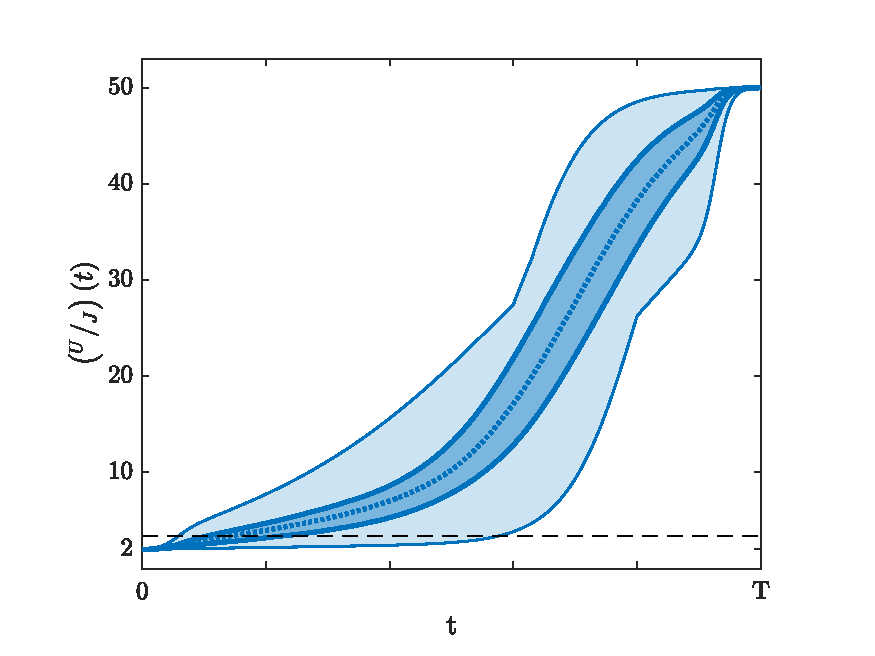
\includegraphics[width=0.7\textwidth]{Figures/LinSigSeed.pdf}
    \caption{\textit{Distribution of seeds used for optimization. All seeds lie within the lightly shaded region, while the darker region contains the 25-75 percentile of seeds. Lastly, the dotted line is the median value of the seed. The dashed line signifies the point of the Bose-Hubbard phase transition.}}
    \label{fig:LinSigSeed}
\end{figure}
Figure \ref{fig:LinSigSeed} shows the distribution of seeds used for the optimizations. Due to control parameter being the interaction strength of the Bose-Hubbard model, the phase transition occurs at quite a low control value. Hence, the initial part of the seed is a slowly increasing linear ramp, which crosses the point of the phase transition with a small slope. A shape function has been multiplied to the seeds enforcing a horizontal slope at the start and end of the duration, which helps avoiding any kinks in the control curve.


\subsection{Tensor Truncation}
A central operation in tensor network calculations is the singular value decomposition or Schmidt decomposition. From the entries of the resulting diagonal eigenmatrix, eigenstates with only little contribution to the current state can be inferred. These states can be discarded with minimal loss of accuracy of the tensorial representation. Discarding eigenstates effectively constitutes a truncation of the tensor bond dimension, whereby one avoids their otherwise exponential scaling. The two central parameters for the truncation are the maximum bond dimension, $D$, and the threshold (or conversely error) for when a state is discarded, $\epsilon_t$.
As discussed in ..... the entanglement entropy increases rapidly around the point of the phase transition. Therefore, the bond dimension required to describe a ground state near the critical point is much higher than otherwise needed for the system. As the system is quenched, the initial ground state decays into a superposition of many eigenstates, whereby the truncation error will rise if a maximum bond dimension is kept \cite{Daley2004}. Therefore, the system is not in the ground state during the phase transition.

To analyze the dynamical scaling of the bond dimension, a system with $L, N_p = 15$ and truncation threshold $\epsilon_t = 10^{-8}$ was time-evolved using an adiabatic-like ramp shown in figure \ref{fig:BondDimComparison}(a).  
\begin{figure}[h!]
    \centering
    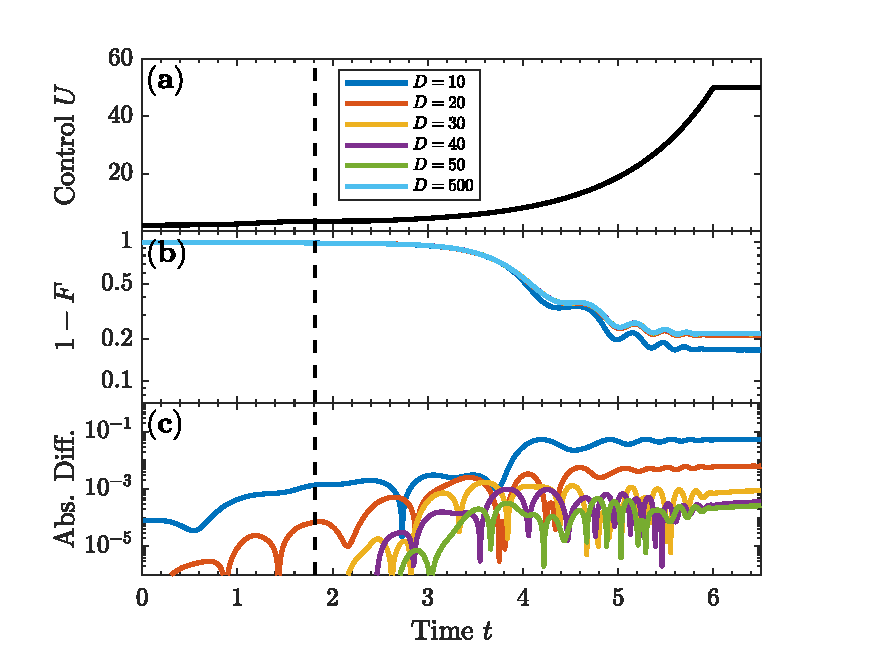
\includegraphics[width=0.7\textwidth]{Figures/BondDim/BondDimComparison.pdf}
    \caption{Ramp sequence for a series of maximum bond dimensions, $D$, and constant truncation threshold $\epsilon_t = 10^{-8}$. The Bose-Hubbard phase transition is marked by a dashed line. \textbf{(a)} the ramp used. \textbf{(b)} infidelities obtained for various values of $D$.  \textbf{(c)} absolute difference in infidelity between non-bounded bond dimension ($D = 500$) and remaining bond dimensions. }
    \label{fig:BondDimComparison}
\end{figure}
Infidelities calculated for various maximum bond dimensions are illustrated in \ref{fig:BondDimComparison}(b-c). Here, the value $D = 500$ has no influence on the bond dimensions, as the truncation is dominated by the threshold. The results obtained for different values of $D$ are very similar initially but starts diverging as time passes. This behavior is expected, as the initial differences between the tensorial representations are amplified during the time-evolution. Nevertheless, the variance in obtained infidelity is relatively small, which confirms the weak scaling with maximum bond dimension reported in \cite{Daley2004}.

To understand the magnitude of the truncations, all the bond dimension of the non-bounded ($D=500$) state are plotted for the ramp duration, which van be seen in figure \ref{fig:BondDimEvolution}(a).
\begin{figure}[h!]
    \centering
    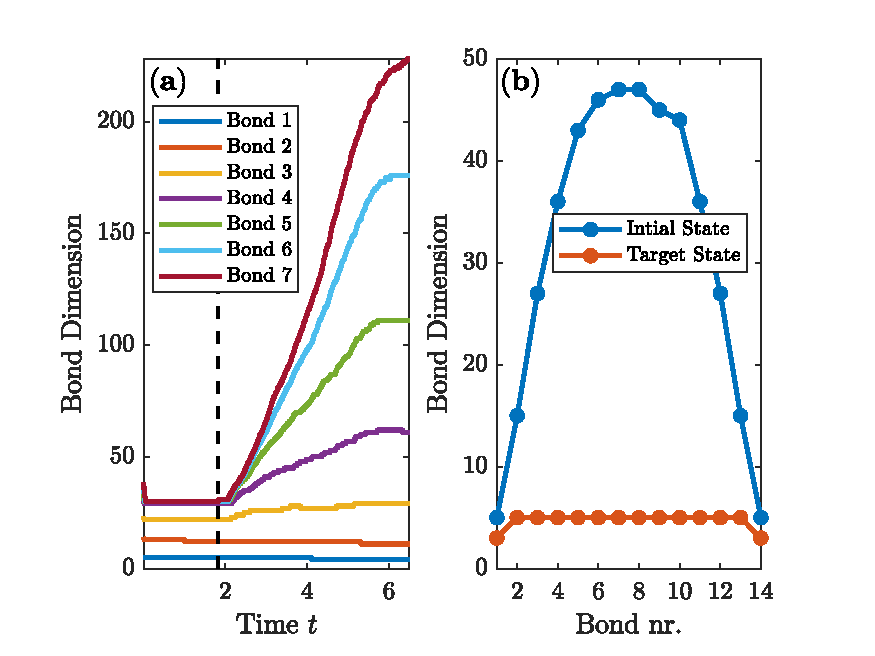
\includegraphics[width=0.7\textwidth]{Figures/BondDim/BondDimEvolution.pdf}
    \caption{Bond dimensions for MPS with $L, N_p = 15$ and $\epsilon_t = 10^{-8}$. \textbf{(a)} evolution of bond dimensions as system is subjected to ramp shown in fig. \ref{fig:BondDimComparison}(a). The dashed line marks the Bose-Hubbard phase transition. \textbf{(b)} bond dimensions of boundary states.}
    \label{fig:BondDimEvolution}
\end{figure}
Initially the bond dimension remains constant, as the ramp is not very steep, whereby the threshold-based truncation keeps the bond dimension stable. At the point of the phase transition the ramp is still almost flat, while the bond dimension suddenly starts increasing rapidly. Although the bond dimension is expected to increase over time \cite{Daley2004}, its sudden increase must be attributed to the large entanglement entropy at the critical point. Unexpectedly, the bond dimensions continue to increase at the same rate for a long time after the phase transition. While this is not completely understood, it can be attributed to either physical dynamics of quasiparticles excited at the critical point \cite{Braun2015}, or mathematical dynamics, as information is propagated at limited speed through tensor network via the Schmidt decompositions.
The bond dimensions of the ground state Mott-Insulator at $U/J = 50$ shown in figure \ref{fig:BondDimEvolution}(b) are much smalled than those of the evolved state at the end of the ramp. Examining the final fidelity displayed in figure \ref{fig:BondDimComparison}(b) reveals that the final state is indeed not in the ground state. Nevertheless, the final bond dimension is remarkably high, but truncating it has only little effect on the fidelity as discussed earlier. Thus, much of the information held in the bond indices at the end of the duration must be redundant, whereby it could be remnants of the phase transition not yet truncated away.

Although the convergence may only scale weakly with the maximum bond dimension, truncating the tensors of the MPS may affect the gradients, which are required to be accurate in order for the L-BFGS approximation to be valid \cite{deFouquieres2011}. 
\begin{figure}[h!]
    \centering
    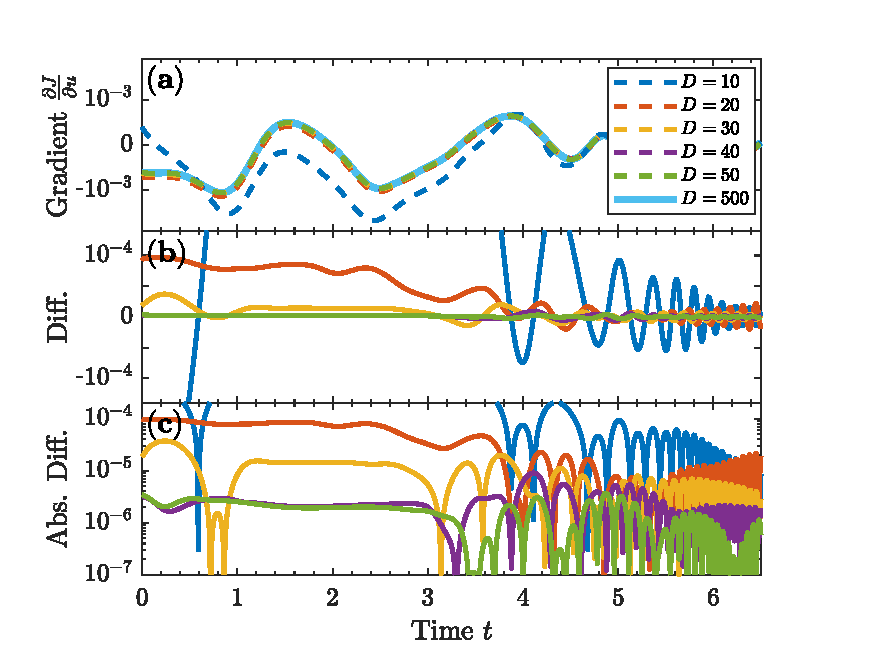
\includegraphics[width=0.7\textwidth]{Figures/BondDim/GradientBondComparison.pdf}
    \caption{\textbf{(a)} GRAPE gradient elements calculated for various maximum bond dimension. \textbf{(b)} difference of derivatives between calculations for $D = 500$ and remaining bond dimensions. \textbf{(c)} absolute differences of derivatives.}
    \label{fig:GradientBondDim}
\end{figure}
Figure \ref{fig:GradientBondDim} shows the results of calculating the gradient elements \ref{eq:STcostgrad} for the ramp shown in figure \ref{fig:BondDimComparison}(a). Compared with the infidelity, the gradient scales more strongly with the maximum bond dimension. Therefore, the truncation is limited by the derivative of the cost function rather than the function itself. Unlike the infidelity, the gradient becomes gradually better during the ramp sequence. The same phenomenon is discussed in section \ref{sec:TrotterGrad} and is caused by the accumulated error when calculating $\ket{\chi (0)}$. Lastly, the gradient shows no signs of being influenced by the phase transition. Thus, gradient-based methods appear to be very well suited for optimal control problems, which involves crossing a critical point.



\section{Characterization of Methods on a Small System} \label{sec:5partOptimization}
To determine suitable settings for the optimization, an initial analysis of a small system consisting of 5 sites with unit occupancy was made. Systems of different sizes are expected to evolve differently, especially due to the closed boundary conditions of the lattice, which have a greater impact for smaller systems. Although the dynamics are expected to vary with the lattice length, certain parameters can be optimized in a smaller system. The regularization factor, $\gamma$, and the dimension of the chopped basis, $M$, only affect the shape of the control pulse, which is subjected to constraints independent of the system size.\\
Due to the small size of the system, no maximum bond dimension was required. Instead, a truncation threshold of $\epsilon_t = 10^{-8}$ was used. Furthermore, the relative tolerance used by the IPOPT library for determining convergence was set at a very low $1e-8$. 

\subsection{Determining the Quantum Speed Limit}
To illustrate the the achieved fidelity's dependence on duration of the control sequence, a series of optimizations were made while scanning over the duration $T$. For this a regularization factor of $\gamma = 10^{-6}$ and an optimization space dimension of $M = 20$ were used. Since the control is parametrized using a linear combination of smooth functions, the effect of the regularization term is limited. Nevertheless, it does help the optimization algorithm avoid greatly varying controls during its initial iterations.\\
Figure \ref{fig:FidelityDuration5} shows the final fidelities obtained for various durations from 100 different initial controls.
\begin{figure}[h!]
    \centering
    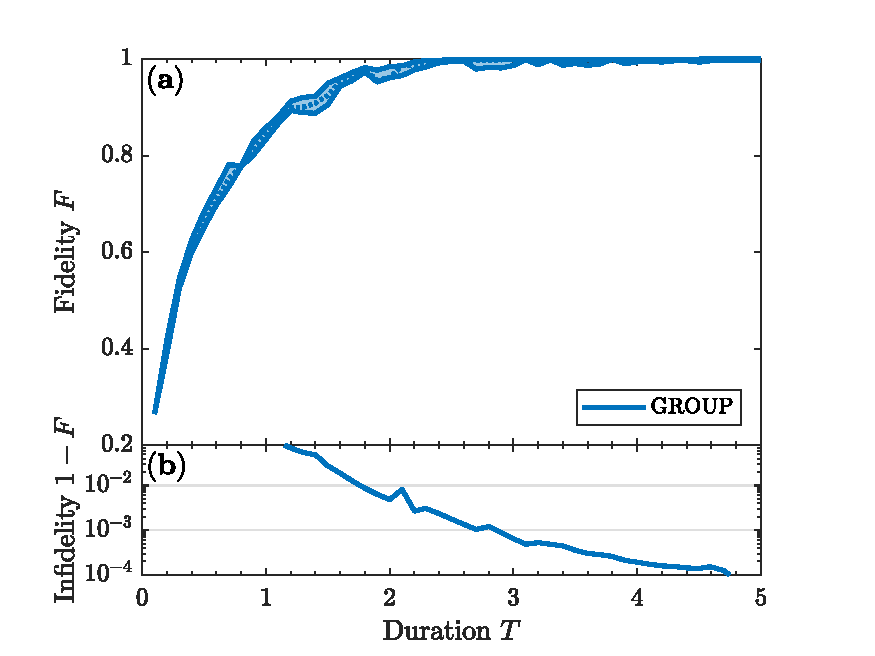
\includegraphics[width=0.8\textwidth]{Figures/5part/FidelityDuration.pdf}
    \caption{\textit{Final fidelity obtained for optimal control at various durations. \textbf{(a)} the dotted line marks the median fidelity achieved, while the shaded area displays the $25\%$- and $75\%$-quartiles of the solutions. \textbf{(b)} the lowest infidelity achieved for each duration. }}
    \label{fig:FidelityDuration5}
\end{figure}
In part \ref{fig:FidelityDuration5}(a) the $25\%$- and $75\%$-quartiles along with the median of the solutions are displayed. At short durations the system can not evolve fast enough from the initial state to reach the target state, hence only low fidelities are obtained. However, as more and more time becomes available, fidelities very close to unit can be reached. Although the final fidelity does not appear to improve beyond $T=3$, figure \ref{fig:FidelityDuration5}(b) reveals the best solutions still improving at longer durations albeit at a reduced rate.\\
Compared to other figures of merit, the fidelity is a very strong measure, as it only considers the overlap with the target state. Due to the large number of quantum states in lattice systems, achieving unit fidelity is practically impossible, and even reaching high fidelities become increasingly difficult with system size. An alternative figure of merit was used for the optimal control of a Bose-Hubbard system presented in \cite{FrankBloch}. Instead of determining the convergence through the infidelity, a rescaled variance of the particle numbers in each of the central sites was used. This figure of merit is much less sensitive to the system size, however, it does have some less favorable properties: First, multiple particle configurations different from unit occupancy of each site can achieve a vanishing particle number variance. Furthermore, the pure state of a single particle on each lattice site only becomes the ground state as the lattice depth tends towards infinity. Therefore, the figure of merit used in \cite{FrankBloch} does not steer the state towards the ground state at the final control value, which could result in residual oscillations of the system after the control sequence. It should be noted that at the final control value used here, the state with a single particle at each site is a very good approximation of the ground state.
Nevertheless, the fidelity is a more direct figure of merit, as it steers the system towards a single, well defined state.\\
Obtaining unit fidelity in a complex quantum system is very difficult, whereby a threshold for accepted final fidelity must be agreed on in order to determine the quantum speed limit. The threshold must be variable with the systems size, due to the sensitivity of the fidelity. In \cite{MajaJulie} a similar optimization was made, and an infidelity threshold of $I_{\mathrm{QSL}} = 10^{-3}$ was set for a 3-site lattice. Adopting the same threshold for the results shown in figure \ref{fig:FidelityDuration5} yields a quantum speed limit of $T_{\mathrm{QSL}}^{(5)} = 2.7$ for the 5-site lattice.\\

Further information regarding the control landscape and the consistency of the algorithm can be inferred from the spread in fidelities shown in figure \ref{fig:FidelityDuration5}.a. A large variety of final fidelities may be due to a control landscape with many local minima. On the other hand, the same phenomenon could be caused by the inability of an algorithm to accurately converge to the minimum. The interior point method is a very robust algorithm capable of handling non-linear constraints, whereby it is reasonable to assume the variations in solutions being caused by the underlying control landscape. Considering the fairly large variation in seeds shown in figure \ref{fig:LinSigSeed}, the control landscape of the 5-site problem must be relatively simple, as the variation in obtained fidelity is rather small.


\subsection{Optimized Ramp Sequences}
A central question is how the optimized ramp sequence differs from its initial seed in both shape and fidelity reached. From figure \ref{fig:FidelityDuration5} one observes that durations around $T = 2.5$ consistently produce solutions with very high fidelity. The lowest infidelities reached at this duration are around $I \approx 10^{-3}$. 
\begin{figure}[h!]
    \centering
    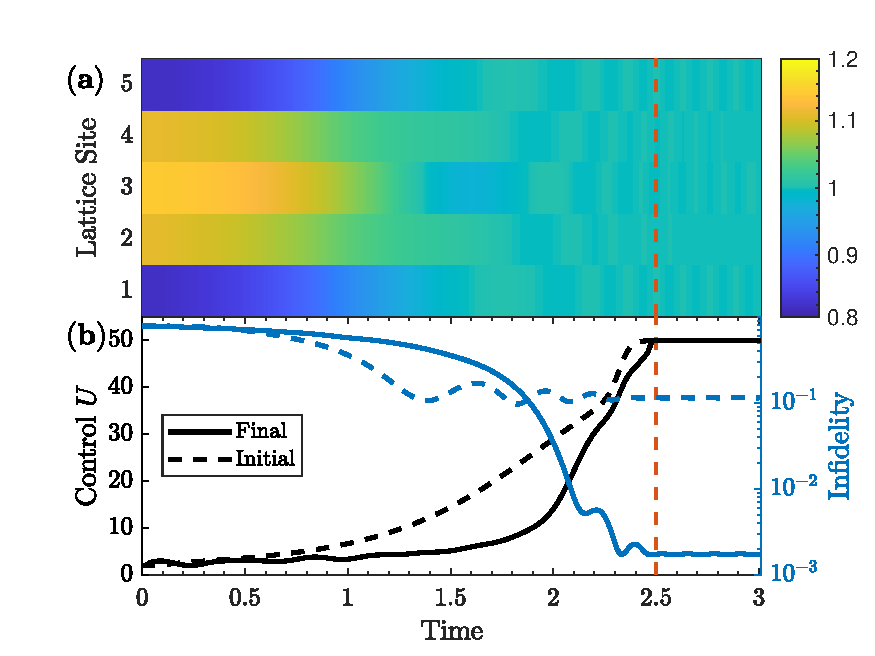
\includegraphics[width=0.8\textwidth]{Figures/5part/ExtendedRampT25.pdf}
    \caption{\textit{Solution with highest fidelity achieved for duration $T = 2.5$. The dashed, red line marks the end of the duration, from which the system is further evolved using the final control value. \textbf{(a)} logarithmically scaled expectation value of the number operator, $\braket{\hat{n}_i}$, for each site as the system is evolved according to the optimized ramp. \textbf{(b)} the initial and optimized ramp sequences along with the corresponding evolution of fidelities.}}
    \label{fig:ExtendedRamp5}
\end{figure}
Figure \ref{fig:ExtendedRamp5} displays an optimized ramp sequence at duration $T = 2.5$ along with an illustration of the evolution of the system. First, consider part \ref{fig:ExtendedRamp5}(b) in which the initial and optimized control is plotted together with the resulting infidelity. Optimizing the initial seed utilizing the GROUP algorithm has resulted in an increase of two magnitudes in the final fidelity achieved.
While the initial ramp is fairly smooth, the optimized ramp wiggles a bit during the first half of the duration followed by a sharp upswing towards the final control value. The steep increase in the control towards the end is very similar to the adiabatic ramp sequence proposed in \cite{Zakrzewski2009}, however, the initial oscillating behavior is non-adiabatic. In fact, examining the optimized ramp sequences for durations shorter than $T = 2.5$ shows an increase in the amplitude of the ramp oscillations, as solutions are required to be increasingly non-adiabatic in order to reach a good fidelity within the given duration. Meanwhile, solutions for durations longer than $T = 2.5$ become increasingly adiabatic-like.\\
After the given optimization duration, $T$, the final control value is kept constant for an additional time span, where the system is further evolved. Any residual evolution of the system at this point is due to the system not being an eigenstate of the Hamiltonian corresponding to final control value. When examining the initial and final ramp sequence after the optimization duration, the initial control appears to reach a more stable state. However, this is an illusion caused by the logarithmic axis, as the optimized ramp produces a state much closer to the target state, which is set as the ground state of $\hat{H}(U(T))$ through the DMRG algorithm.\\ 
Figure \ref{fig:ExtendedRamp5}(a) illustrates the expectation value of the number operator, $\braket{\hat{n}_i}$, for each site during the ramp. Initially the system is in the superfluid state causing a low energetic cost for having multiple particles on each site. Thus, one observes a reduced number of particles at the outer sites of the lattice due to the closed boundary conditions. As the system is evolved towards the Mott-Insulating state, having multiple particles at the same sites becomes very energetically unfavorable. Hence, the target state has a single particle at each site, as it is deep in the Mott regime. The optimized ramp brings the system very close to this configuration of particles, which can be observed near the dashed red line marking the end of the duration, $T$. Some imperfections are present, although their magnitude is exaggerated by the logarithmic color axis. The residual oscillations of the infidelity after the optimization durations can be seen in figure \ref{fig:ExtendedRamp5}(a) as fluctuations of the particle number. 


\subsection{Control Basis Size}
Unlike GRAPE, which takes the full optimization space into account, parameterizations like GROUP utilize a chopped basis resulting in a much smaller dimension of the optimization space. When reducing the dimension of the optimization space through a parametrization as described in eq. \eqref{eq:controlParametrization}, the new control basis must be able to span the solution space. Otherwise artificial minima can be introduced to the control landscape due to the incompleteness of the basis \cite{Rach2015}. 
In the implementation of GROUP used for these calculations, the basis functions of the chopped basis are of the form $f_n = \sin \left( \omega_n t / T \right)$, where $\omega_n = n \pi$.
To investigate the basis size required to describe the optimal solutions, a series of optimizations were made for various basis sizes at the duration $T = 2.5$. 
\begin{figure}[h!]
    \centering
    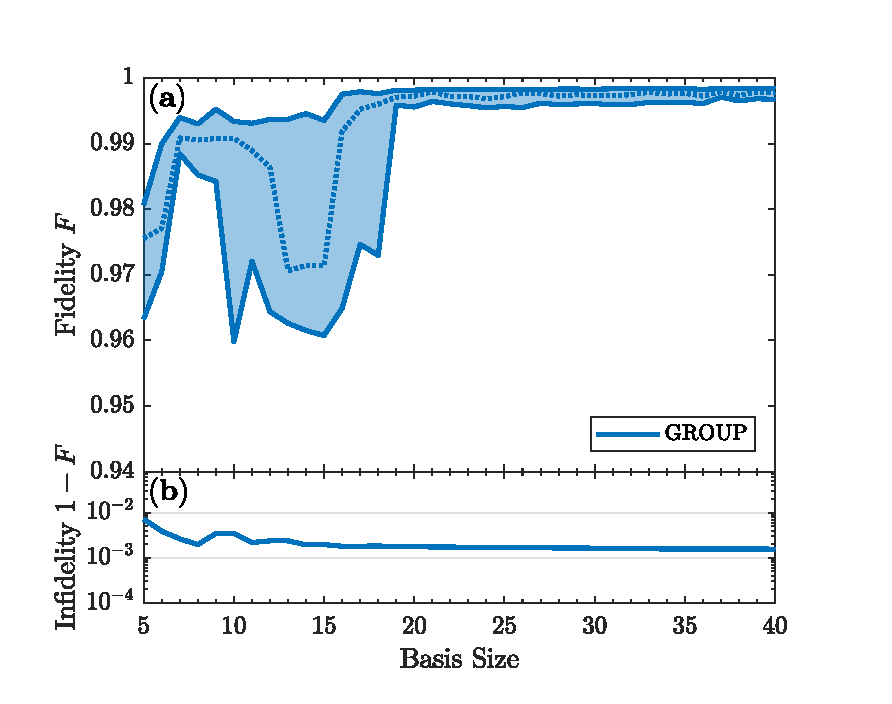
\includegraphics[width=0.8\textwidth]{Figures/5part/BestFidelityBasisSize.pdf}
    \caption{\textit{Final fidelity obtained for optimal control at various optimization space dimensions for duration $T = 2.5$. \textbf{(a)} the dotted line marks the median fidelity achieved, while the shaded area displays the $25\%$- and $75\%$-quartiles of the solutions. \textbf{(b)} the lowest infidelities achieved for each basis size.}}
    \label{fig:FidelityBasisSize5}
\end{figure}
The results of the scan over the basis size can be seen in figure \ref{fig:FidelityBasisSize5}. From figure \ref{fig:FidelityBasisSize5}(a) it is evident that a basis size of around 20 and above consistently produces high-fidelity solutions, while the quality of solutions using a smaller basis size fluctuated greatly. Thus, high-fidelity ramps for $T = 2.5$ have at least 20 frequency components. Although results obtained with a smaller basis are generally worse, high fidelity solutions are still possible to achieve, as the optimal solution may still be realizable using only few frequencies. This can be observed in figure \ref{fig:FidelityBasisSize5}(b), where the infidelity of the best solution remains constant, while the median fidelity of the solutions decreases. The large spread in final fidelity is a consequence of a more complicated optimization landscape with artificial minima.


\section{Optimal Control of Large Lattice Systems} \label{sec:20partOptimization}